% CVPR 2022 Paper Template
% based on the CVPR template provided by Ming-Ming Cheng (https://github.com/MCG-NKU/CVPR_Template)
% modified and extended by Stefan Roth (stefan.roth@NOSPAMtu-darmstadt.de)
\documentclass[10pt,twocolumn,letterpaper]{article}
%%%%%%%%% PAPER TYPE  - PLEASE UPDATE FOR FINAL VERSION
%\usepackage[review]{cvpr}      % To produce the REVIEW version
%\usepackage{cvpr}              % To produce the CAMERA-READY version
\usepackage[pagenumbers]{cvpr} % To force page numbers, e.g. for an arXiv version
% Include other packages here, before hyperref.
\usepackage{algorithm}
\usepackage{algorithmic}
\usepackage{graphicx}
\usepackage{amsmath}
\usepackage{amssymb}
\usepackage{booktabs}
\usepackage{adjustbox}
% It is strongly recommended to use hyperref, especially for the review version.
% hyperref with option pagebackref eases the reviewers' job.
% Please disable hyperref *only* if you encounter grave issues, e.g. with the
% file validation for the camera-ready version.
%
% If you comment hyperref and then uncomment it, you should delete
% ReviewTempalte.aux before re-running LaTeX.
% (Or just hit 'q' on the first LaTeX run, let it finish, and you
%  should be clear).
\usepackage[pagebackref,breaklinks,colorlinks]{hyperref}
\usepackage{hyperref} % Import the hyperref package

% Support for easy cross-referencing
\usepackage[capitalize]{cleveref}
\crefname{section}{Sec.}{Secs.}
\Crefname{section}{Section}{Sections}
\Crefname{table}{Table}{Tables}
\crefname{table}{Tab.}{Tabs.}
%%%%%%%%% PAPER ID  - PLEASE UPDATE
\def\cvprPaperID{00000} % *** Enter the CVPR Paper ID here
\def\confName{CVPR}
\def\confYear{2023}


\begin{document}
	
	%%%%%%%%% TITLE - PLEASE UPDATE
	\title{Enhancing LiDaR semantic segmentation using model soups }
	\author{ Omar Wasfy\\
	{\tt\small omar.wasfy@alexu.edu.eg}
\and
Marwan Torki\\
{\tt\small mtorki@alexu.edu.eg}
\and
Sohier Basiony\\
{\tt\small sohier.basiony@alexu.edu.eg}
}
\maketitle

%%%%%%%%% ABSTRACT
\begin{abstract}
	In this paper, we present a pioneering approach for model soups \cite{wortsman2022model,dansereau2023model}, named "Iterative Scan Greedy Model Soup," and apply it to the domain of LiDAR semantic segmentation. using this technique, we augment the state-of-the-art open source code for 2DPASS \cite{yan20222dpass} semantic segmentation and demonstrate its efficacy on both the semanticKitti dataset and the nuscenes dataset. Remarkably, our approach achieves improvements in Mean Intersection Over Union (MIoU) without any increase in prediction time, all while retaining the original model structure.	Our contributions in this work are described in two points: Firstly, we successfully extend the application of model soups to LiDAR semantic segmentation, showcasing their adaptability and potential impact on the domain. Second, we introduce an optimized and efficient version of the existing greedy soup technique, further enhancing the overall performance of the approach. Through comprehensive experiments and rigorous evaluations, our results highlight the significance of the iterative scan greedy model soup in advancing LiDAR semantic segmentation, opening up new possibilities for enhanced perception systems in autonomous driving and related fields.
\end{abstract}

%%%%%%%%% BODY TEXT
\section{Introduction}
\label{sec:intro}

In recent years, semantic segmentation of LiDAR point clouds has emerged as a critical area of research, especially in advancing the scene-understanding capabilities of self-driving cars.\cite{hu2019randla,yan2021sparse,SparseConv} The methods for semantic segmentation of LiDAR point clouds can be categorized based on their input modalities into two main groups:

Single Modality LiDAR-Based Input: These methods depend only on LiDAR data as input. However, due to the sparse nature of LiDAR input, such single-modality-only approaches often face challenges in accurately segmenting complex scenes.\cite{chen2017deeplab,chen2017rethinking,song2017semantic,huang2019ccnet,yan2021sparse,xu2020squeezesegv3,zhu2021cylindrical,tang2020searching,zheng2022beyond,zheng2021box}

Multiple-Modality LiDAR-Based and Camera-Based Input: These methods use both LiDAR-based and camera-based inputs. By fusing information from both modalities, these techniques attempt to exploit the strengths of each sensor to achieve more robust semantic segmentation.\cite{zhuang2021perception,el2019rgb,vora2020pointpainting}

The open-source model "2D Priors Assisted Semantic Segmentation" (2DPASS)\cite{yan20222dpass} utilizes multiple modalities during the training process to enhance the prediction capabilities of a single-modality model. However, after training, only the single modality (LiDAR) is retained, making it a more practical solution in real-world deployment.

In the context of model ensembling, Model soups present an efficient approach for improving model performance without modifying the underlying model structure. This technique involves creating an ensemble of models with uniform structures and achieving performance gains akin to traditional ensembling methods without incurring additional prediction costs.

Building on the foundation of 2DPASS \cite{yan20222dpass}, we propose a novel enhancement to the approach. We introduce a procedure where multiple checkpoints are saved during the training process, and subsequently, a new round of optimization is performed using model soups techniques. By iteratively applying model soups, we aim to further enhance the predictive capabilities of the LiDAR-based single-modality model.

In this paper, we present our iterative scan greedy model soup approach, which leverages the strengths of both 2DPASS \cite{yan20222dpass} and model soups. We demonstrate the effectiveness of our method by conducting extensive experiments on LiDAR semantic segmentation tasks. The results showcase the potential of our approach to achieve notable performance improvements without altering the original model architecture and without incurring additional prediction time.

The contributions of this work are: \\ 
  \begin{enumerate}
\item Our work involves the integration of model soups with 2DPASS \cite{yan20222dpass}, offering a fresh perspective for enhancing single-modality LiDAR-based semantic segmentation models. To the best of our knowledge, no previous research has explored the application of the model souping technique to the task of LiDAR modality segmentation.

\item The validation of our iterative scan greedy model soup approach through various experiments demonstrates its substantial value in improving semantic segmentation, particularly for enhancing scene understanding in the context of self-driving cars.
\end{enumerate}




%-------------------------------------------------------------------------
\section{Related Work}
\subsection{ Single-Sensor Methods
}

\subsubsection{Camera-Based Methods:}
These methods aim to predict pixel-wise labels for 2D images, with FCN \cite{long2015fully} being a pioneering architecture in this field. Recent advancements have explored multi-scale feature learning, dilated convolution, and attention mechanisms to achieve significant improvements. However, camera-only methods suffer from limitations in depth sensing and low-light conditions.\cite{he2016deep,chen2017rethinking,chen2017deeplab,lin2016efficient,zhao2017pyramid,wang2018understanding,huang2019ccnet,yuan2018ocnet}

\subsubsection{LiDAR-Based Methods:}
These methods process LiDAR point clouds directly. Point-based methods, like PointNet \cite{qi2016pointnet}, utilize per-point Multi-Layer Perceptron (MLP)\cite{rosenblatt1958perceptron} While these methods extract local features from point clouds, they can be inefficient due to time-consuming sampling and grouping algorithms.\cite{thomas2019kpconv,qi2017pointnet++,wang2019dynamic,PointConv,liu2019relation,Thomas_2019_ICCV,hua2018pointwise,yan2020pointasnl,zhao2021point,engel2021point,yan2020pointasnl,zhao2021point,engel2021point}


\subsubsection{Projection-based methods}
These methods project LiDAR point clouds onto 2D pixels, allowing the use of traditional CNNs. However, such methods suffer from information loss, leading to lower segmentation accuracy \cite{lawin2017deep, boulch2017unstructured, tatarchenko2018tangent,wu2018squeezeseg,wu2019squeezesegv2,liong2020amvnet}.

\subsubsection{Voxel-based frameworks}
These methods using SparseConv \cite{SparseConv}, have become popular due to their efficiency. These methods store only nonempty voxels in a Hash table and perform convolution operations more efficiently. Recent studies have utilized SparseConv \cite{?} to design powerful network architectures, but they still face challenges in achieving higher segmentation accuracy \cite{zhou2020cylinder3d,cheng20212}.

\subsection{Multi-Sensor Methods}

These methods aim to combine information from both cameras and LiDAR, taking advantage of the strengths of both modalities. 
Approaches like RGBAL \cite{el2019rgb} convert RGB images to polar-grid mapping representations and use early and mid-level fusion strategies. 
PointPainting \cite{vora2020pointpainting}  improves LiDAR network performance by projecting segmentation logits from images into the LiDAR space. 
PMF \cite{zhuang2021perception} explores the collaborative fusion of two modalities in camera coordinates. However, these methods require multi-sensor inputs during both training and inference, making them computationally intensive and less practical for real-world applications.\cite{krispel2020fuseseg,el2019rgb,meyer2019sensor,vora2020pointpainting}

\subsection{Cross-modal Knowledge Transfer}

Knowledge distillation \cite{hinton2015distilling}, initially was for model compression, has been extended to transfer knowledge between different models through the alignment of feature representations.\cite{ba2013deep,chen2017learning,zagoruyko2016paying,srinivas2018knowledge,gupta2016cross,wang2019efficient,yuan2018rgb,liu20213d,zhao2020knowledge}
Recently, knowledge distillation has been applied to transfer priors across different modalities, using extra 2D images during training to improve inference performance. 
Various approaches have been explored, such as 2D-assisted pre-training  \cite{liu2021learning}, 
inflating 2D convolution kernels to 3D \cite{xu2021image2point}, 
and well-designed teacher-student frameworks \cite{yuan2022x}.

In this work, we introduce a novel model soup \cite{wortsman2022model,dansereau2023model} technique applicable to all the above methods because of its inherent model-agnostic feature. 
This technique improves the results without changing the model architecture or incurring extra processing time. By leveraging the complementary information from 2D images, our method improves the segmentation accuracy of LiDAR point clouds in a cross-modal setup. We believe this approach can be a valuable addition to the existing methods for multi-sensor semantic segmentation and also in other machine learning-based methods.
%-------------------------------------------------------------------------


\section{ Approach }
Model souping \cite{wortsman2022model,dansereau2023model} is an ensemble learning technique that averages the weights of multiple models to create a single, more accurate, and robust model. This approach can help mitigate overfitting and improve generalization performance. Model souping is different from traditional ensemble learning techniques in that it averages the weights of models, rather than their predictions. This can help to improve the diversity of the ensemble and reduce the risk of overfitting. Model souping can be computationally expensive and requires more training data than traditional ensemble learning techniques. However, it can offer significant performance improvements over traditional methods.
\begin{table}[!h]
\centering\
\small
\begin{tabular}{p{3.5cm} p{4cm}}
		\toprule
		\textbf{Method} & \textbf{Description} \\
		\midrule
		Best ValAcc Model & Choose model with highest validation accuracy ValAcc($\theta_i$) \\
		Ensemble & Combine predictions of models parameterized by $\theta_i$ \\
		Uniform Soup & Average parameter values $\theta_i$ \ \cite{wortsman2022model} \\
		Greedy Soup & Greedy approach for the model ensemble \cite{wortsman2022model}\\
		Learned Soup & Learn optimized ensemble of models \cite{wortsman2022model} \\
		Pruned Soups & Select subset of models for ensemble \cite{dansereau2023model} \\
		Iterative Uniform Greedy Soup Alg. 1 & Iterative Greedy Soup with Uniform Weights \\
		\bottomrule
	\end{tabular}
	\caption{Summary of Methods}
\end{table}
\begin{algorithm}[!h]
\caption{Iterative Uniform Greedy Soup}
\label{alg:algorithm}
\textbf{Input}: weights of Potential soup ingredients ${\theta_1, ..., \theta_k}$ (optionally sorted in decreasing order of \textbf{ValAcc}($\theta_i$))\\
\textbf{Parameter}:epochs\\
\begin{algorithmic}[1] %[1] enables line numbers
\STATE soupList = emptyList
\STATE bestValAcc = 0
\FOR{epoch=1 to epochs}
\FOR{i=1 to k}
\STATE potentialSoupList $\leftarrow$ AddToSoupList($\theta_i$)
\IF {\textbf{ValAcc}(potentialSoupList) $>=$ bestValAcc}
\STATE bestValAcc = \textbf{ValAcc}(potentialSoupList)
\STATE soupList $\leftarrow$ potentialSoupList
\ENDIF
\ENDFOR
\ENDFOR
\STATE \textbf{return} weights of the final soup $\theta_{soupList}$
\end{algorithmic}
\end{algorithm}
\section{Experiments}
\subsection{Experiment setup}
we have collected 100 checkpoints of while training 2DPASS \cite{yan20222dpass} on both  Semantickitti \cite{behley2019semantickitti}. and Nuscenes \cite{caesar2020nuscenes}  datasets.
We have applied our modified greedy soup technique
also we have conducted a comparison between collected checkpoints  class-wise and average miou performance using tta with number of votes = 12 and showed the improvement of using tta against non-tta in semantic Kitti validation set for collected checkpoints while training   
\subsection{Results}.
\begin{table}[!h]
\centering
\small
	\caption{Semantic Kitti Performance Metrics for Different Objects/Models}
	\begin{tabular}{{p{3cm} p{0.5cm} p{0.5cm} p{0.5cm} p{0.5cm} p{0.5cm} p{0.5cm} p{0.5cm}}}
		\toprule
		Objects/Models & Best & Best TTA & Paper Best & Paper Best TTA & 13 Ingredients & 24 Ingredients TTA & 24 Ingredients \\
		& Indiv. & Indiv. & & & & TTA & \\
		& Model & Model & & & & & \\
		\midrule
		car & 96.12 & 96.98 & 96.83 & 97.26 & 96.44 & 97.26 & 96.51 \\
		bicycle & 49.04 & 53.02 & 52.55 & 55.25 & 49.73 & 54.42 & 49.75 \\
		motorcycle & 73.68 & 76.69 & 76.31 & 78.72 & 71.89 & 76.28 & 72.36 \\
		truck & 79.11 & 92.5 & 90.75 & 90.79 & 84.94 & 95.34 & 85.22 \\
		bus & 64.24 & 70.85 & 71.38 & 72.08 & 68.06 & 74.69 & 69.22 \\
		person & 73.66 & 77.98 & 78.35 & 80.74 & 75.08 & 78.83 & 75.09 \\
		bicyclist & 87.8 & 91.41 & 92.35 & 93.55 & 88.77 & 92.97 & 89.16 \\
		motorcyclist & 0.19 & 0 & 0.06 & 0.14 & 0 & 0 & 0 \\
		road & 92.48 & 93.96 & 93.24 & 94.31 & 92.43 & 93.9 & 92.34 \\
		parking & 45.01 & 50.93 & 50.75 & 53.77 & 44.03 & 47.45 & 43.36 \\
		sidewalk & 78.84 & 81.53 & 80.08 & 82.03 & 78.95 & 81.56 & 78.81 \\
		other-ground & 4.81 & 7.32 & 8.44 & 12.09 & 5.2 & 7.19 & 5.44 \\
		building & 90.8 & 91.9 & 92.21 & 93 & 91.42 & 92.54 & 91.5 \\
		fence & 61.4 & 66.35 & 68.27 & 71.61 & 63.61 & 69.1 & 63.92 \\
		vegetation & 88.28 & 89.4 & 88.37 & 89.11 & 88.38 & 89.59 & 88.54 \\
		trunk & 70.71 & 73.17 & 71.19 & 72.23 & 70.98 & 72.62 & 70.93 \\
		terrain & 75.11 & 76.69 & 74.64 & 75.72 & 75.41 & 77.38 & 75.92 \\
		pole & 58.8 & 63.94 & 63.92 & 66.06 & 59.73 & 64.25 & 59.9 \\
		traffic-sign & 50.23 & 53.16 & 53.46 & 54.26 & 50.33 & 51.99 & 50.13 \\
		\midrule
		AVG mIoU uniform & 65.28 & 68.83 & 68.59 & 70.14 & 66.07 & 69.33 & 66.22 \\
		val/best\_miou & 65.88 & 69.22 & 68.63 & 70.16 & 66.54 & 69.55 & 66.71 \\
		val/mIoU & 65.28 & 68.83 & 68.59 & 70.14 & 66.07 & 69.34 & 66.22 \\
		val/acc & 88.87 & 89.88 & 89.36 & 90.01 & 89.03 & 90.04 & 89.09 \\
		\bottomrule
	\end{tabular}
\end{table}
\begin{table}[!h]
	\centering
	\small
	\caption{Nuscenes Performance Metrics for Different Objects/Models}
	\begin{tabular}{{p{3cm} p{1cm} p{1cm} p{1cm} p{1cm}}}
		\toprule
		Objects/Models & Best Individual & Best Paper & Best Paper TTA & 16 Ingredients \\
		& Model & Model & & \\
		\midrule
		movable\_object.barrier & 74.59 & 75.4 & 77.86 & 74.67 \\
		vehicle.bicycle & 36.27 & 42.48 & 50.37 & 36.28 \\
		vehicle.bus.bendy & 93.85 & 95.11 & 95.91 & 94.73 \\
		vehicle.car & 92.07 & 90.71 & 92.12 & 91.45 \\
		vehicle.construction & 53.95 & 57.39 & 61.38 & 55.08 \\
		vehicle.motorcycle & 80.88 & 85.65 & 87.97 & 81.72 \\
		human.pedestrian.adult & 78.15 & 78.65 & 81.84 & 78.21 \\
		movable\_object.trafficcone & 55.68 & 61.48 & 66.91 & 56.34 \\
		vehicle.trailer & 70.63 & 65.86 & 73.21 & 71.14 \\
		vehicle.truck & 86.77 & 86.04 & 89.27 & 87.55 \\
		flat.driveable\_surface & 96.04 & 96.08 & 96.68 & 96.11 \\
		flat.other & 71.75 & 73.02 & 74.74 & 73.04 \\
		flat.sidewalk & 73.4 & 73.15 & 75.12 & 73.76 \\
		flat.terrain & 73.82 & 73.84 & 75.56 & 74.28 \\
		static.manmade & 87.71 & 87.44 & 88.6 & 87.74 \\
		static.vegetation & 85.78 & 85.58 & 86.84 & 86.11 \\
		\midrule
		AVG mIoU uniform & 75.71 & 76.74 & 79.65 & 76.14 \\
		val/best\_miou & 77.41 & 78.31 & 81.26 & 77.81 \\
		val/mIoU & 75.71 & 76.74 & 79.65 & 76.14 \\
		val/acc & 61.80 & 61.76 & 62.22 & 61.87 \\
		\bottomrule
	\end{tabular}
\end{table}


\begin{table}[!h]
\centering
\begin{tabular}{l l}
\hline
\textbf{Checkpoint} & \textbf{MIoU} \\
\hline
Best individual checkpoint & 62.7293496631 \\
Best individual checkpoint with TTA=12 & 65.7479476497 \\
Enhanced Greedy Soup without early stopping & 62.9877710884 \\
Enhanced Greedy Soup with early stopping & 63.1813711987 \\
Enhanced Greedy Soup with early stopping with TTA=24 & 65.7048807097 \\
Enhanced Greedy Soup with early stopping with TTA=12 & 65.6100402842 \\
Normal greedy soup & 65.4171732912 \\
Paper Github best provided checkpoint with TTA=1 & 65.2979295686 \\
\hline
\end{tabular}
\caption{Testing Results on SemanticKitti MIoU for Different Checkpoints}
\label{tab:miou_results}
\end{table}



\begin{enumerate}
\item Using Test-Time Augmentation (TTA), Greedy Soup shows a slightly lower performance compared to the best individual checkpoint from training. Specifically, with Greedy Soup using TTA=24, the performance is 0.04% lower, and with TTA=12, it's 0.1% lower.

\item We can observe that Greedy Soup performs better without Test-Time Augmentation, which is a form of ensembling. This result contrasts with the validation set, indicating a possible overfitting pattern. During the attempt to assemble the best combination of ingredients to enhance validation mIoU, there might have been a tendency to slightly overfit the validation dataset. Interestingly, Greedy Soup's model performs better than the best checkpoint in testing with TTA=1, suggesting an improvement in generalization capacity and indicating that Greedy Soup's model has enhanced without overfitting.
\end{enumerate}

\subsection{Analysis of collected Semantic Kitti checkpoints}



\begin{table}[!h]
\centering
\begin{tabular}{l c}
\hline
Class & Avg mIoU \\
\hline
car & 0.9661 \\
road & 0.9335 \\
truck & 0.8381 \\
building & 0.9130 \\
bicyclist & 0.8977 \\
vegetation & 0.8928 \\
sidewalk & 0.8011 \\
person & 0.7626 \\
terrain & 0.7698 \\
motorcycle & 0.7177 \\
trunk & 0.7164 \\
bus & 0.6517 \\
fence & 0.6379 \\
pole & 0.6256 \\
traffic-sign & 0.5171 \\
bicycle & 0.5050 \\
parking & 0.4611 \\
other-ground & 0.0483 \\
motorcyclist & 0.0046 \\
\hline
\end{tabular}
\caption{Average mIoU Scores for Different Classes for semanticKitti Checkpoints}
\label{tab:miou_scores}
\end{table}

\begin{figure}[!h]
    \centering
    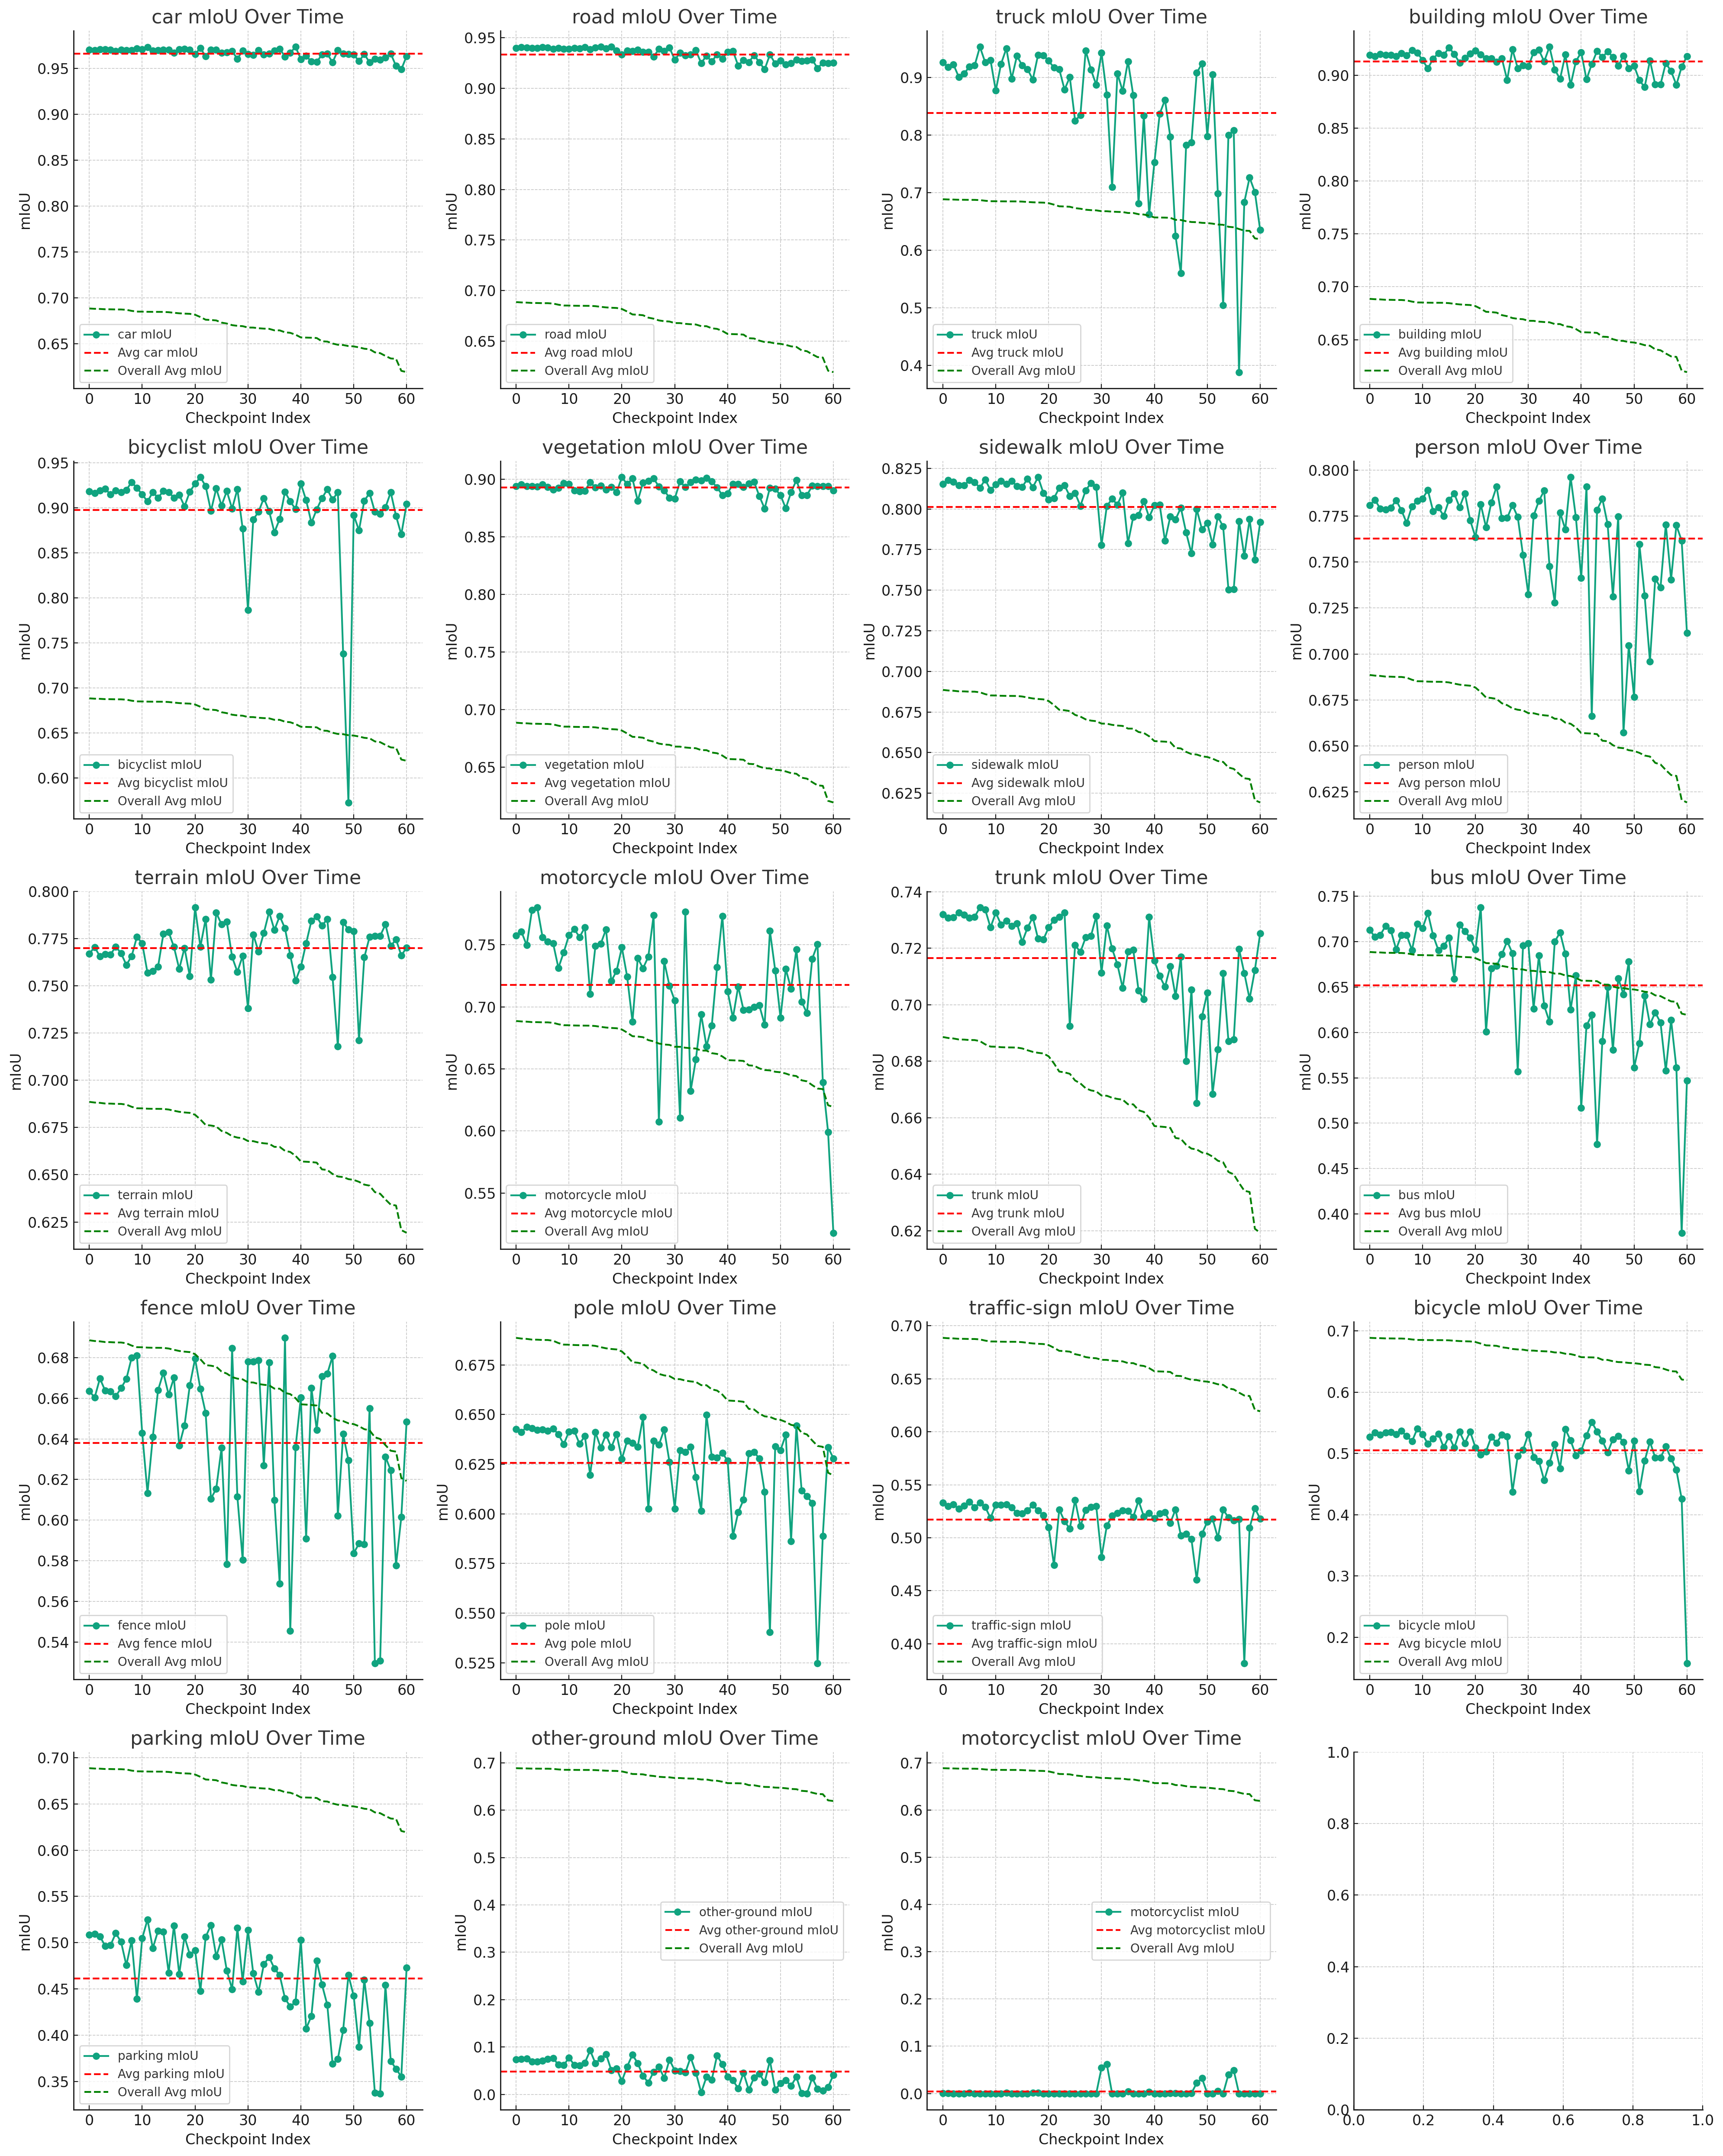
\includegraphics[width=0.5\textwidth]{photos/class miou vs epoch ordered by average miou desc.png}
    \caption{The subplots present the mIoU progression for each semantic class across checkpoints. The blue line plots the mIoU scores at each checkpoint, while the red dashed line indicates the class-specific average mIoU, and the green dashed line represents the overall average mIoU across all classes and checkpoints. This visualization aids in understanding both temporal and comparative performance metrics for each class.}
    \label{fig:photo_example}
\end{figure}



\begin{figure}[!h]
    \centering
    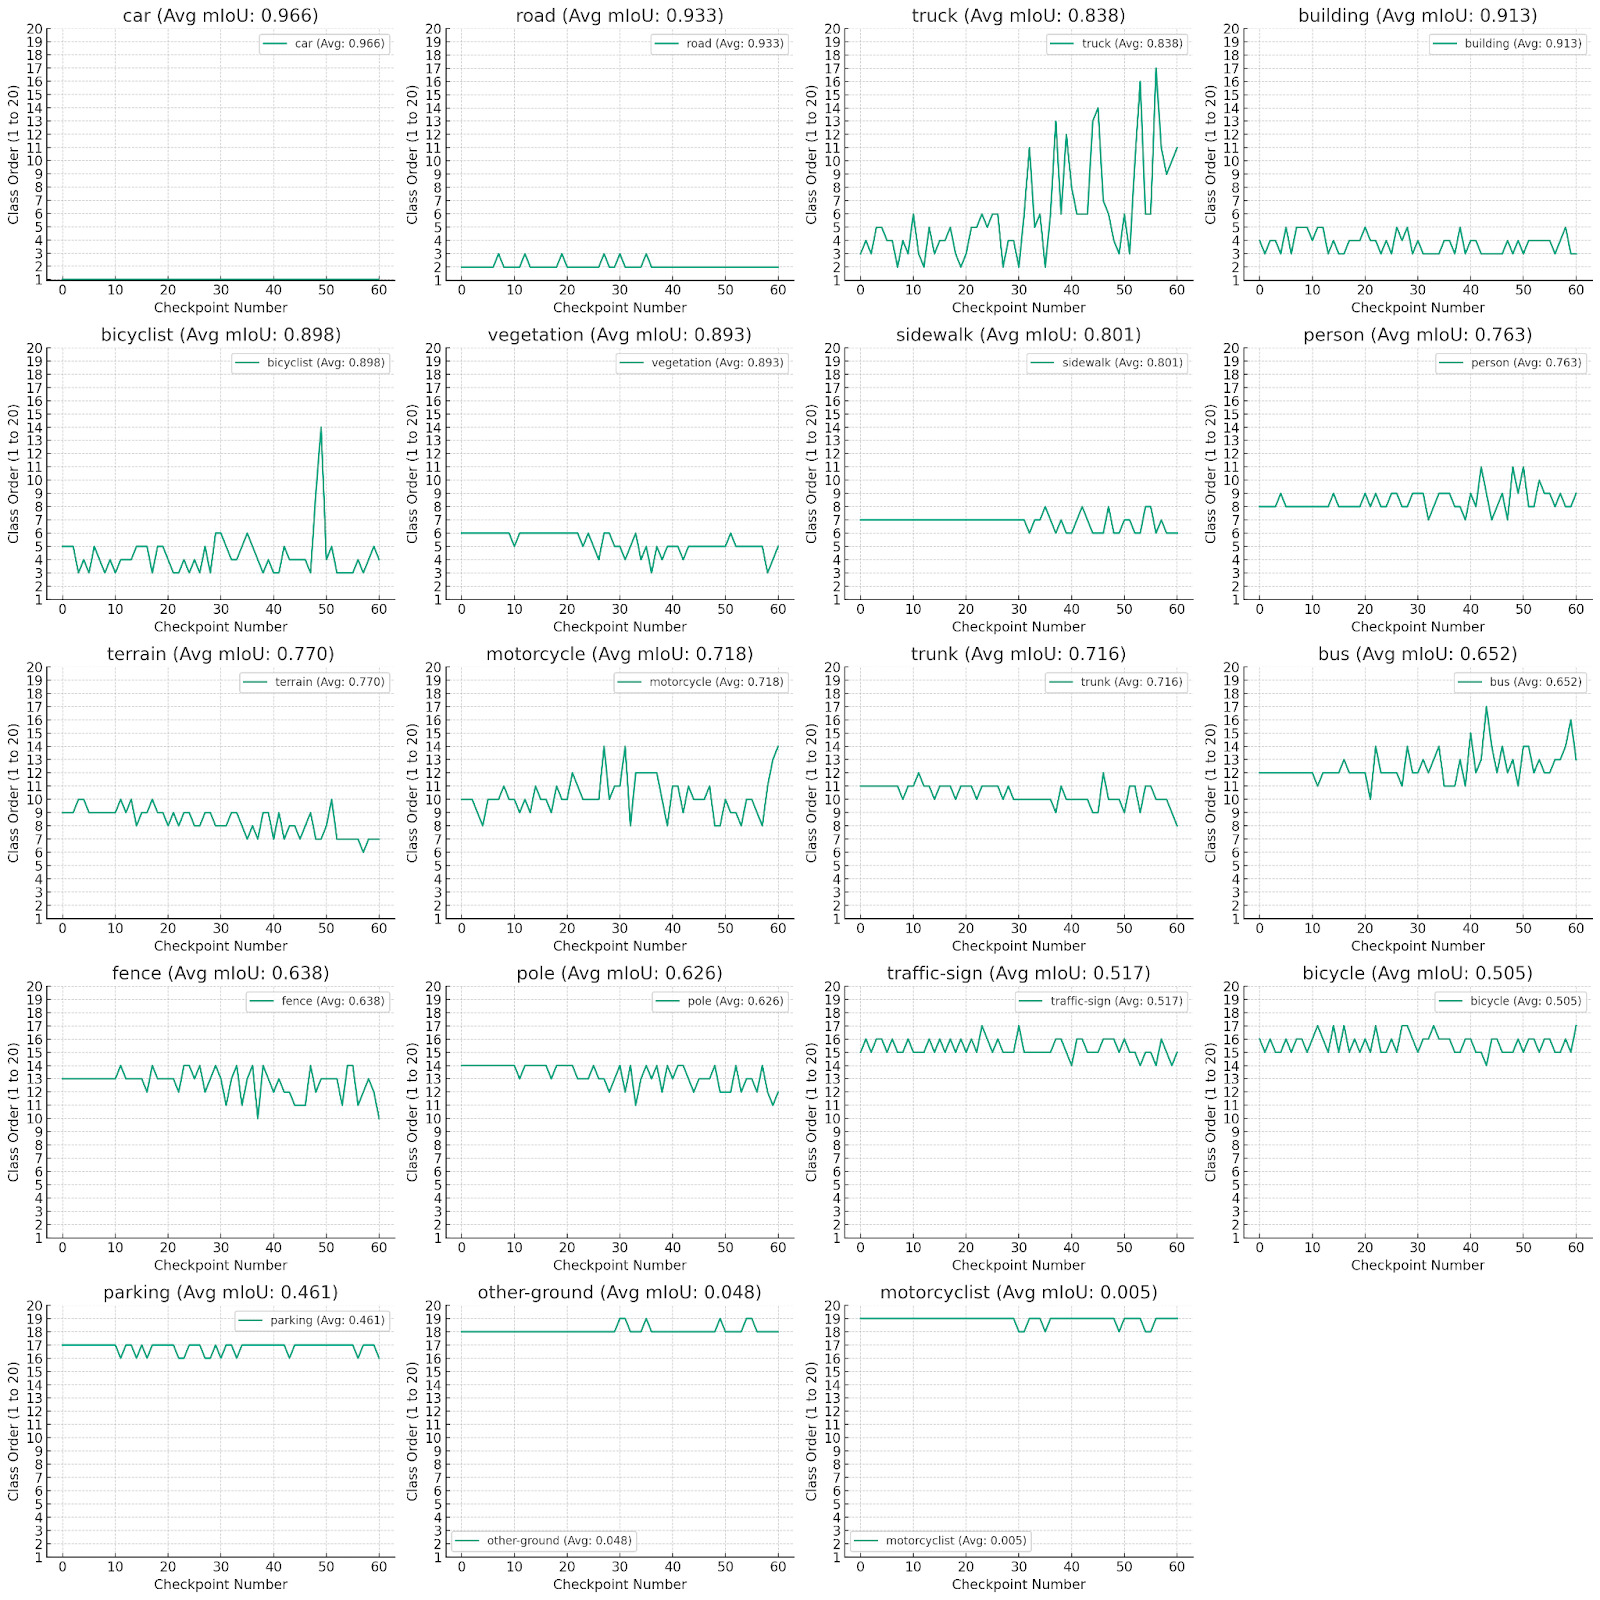
\includegraphics[width=0.5\textwidth]{photos/class ordering accross semantickitti checkpoints.png}
    \caption{Class ordering through collected semanticKitti ordered with respect to average miou of all classes training checkpoints , checkpoint 0 is the best performing average miou checkpoint  }
    \label{fig:photo_example}
\end{figure}

\begin{figure}[!h]
    \centering
    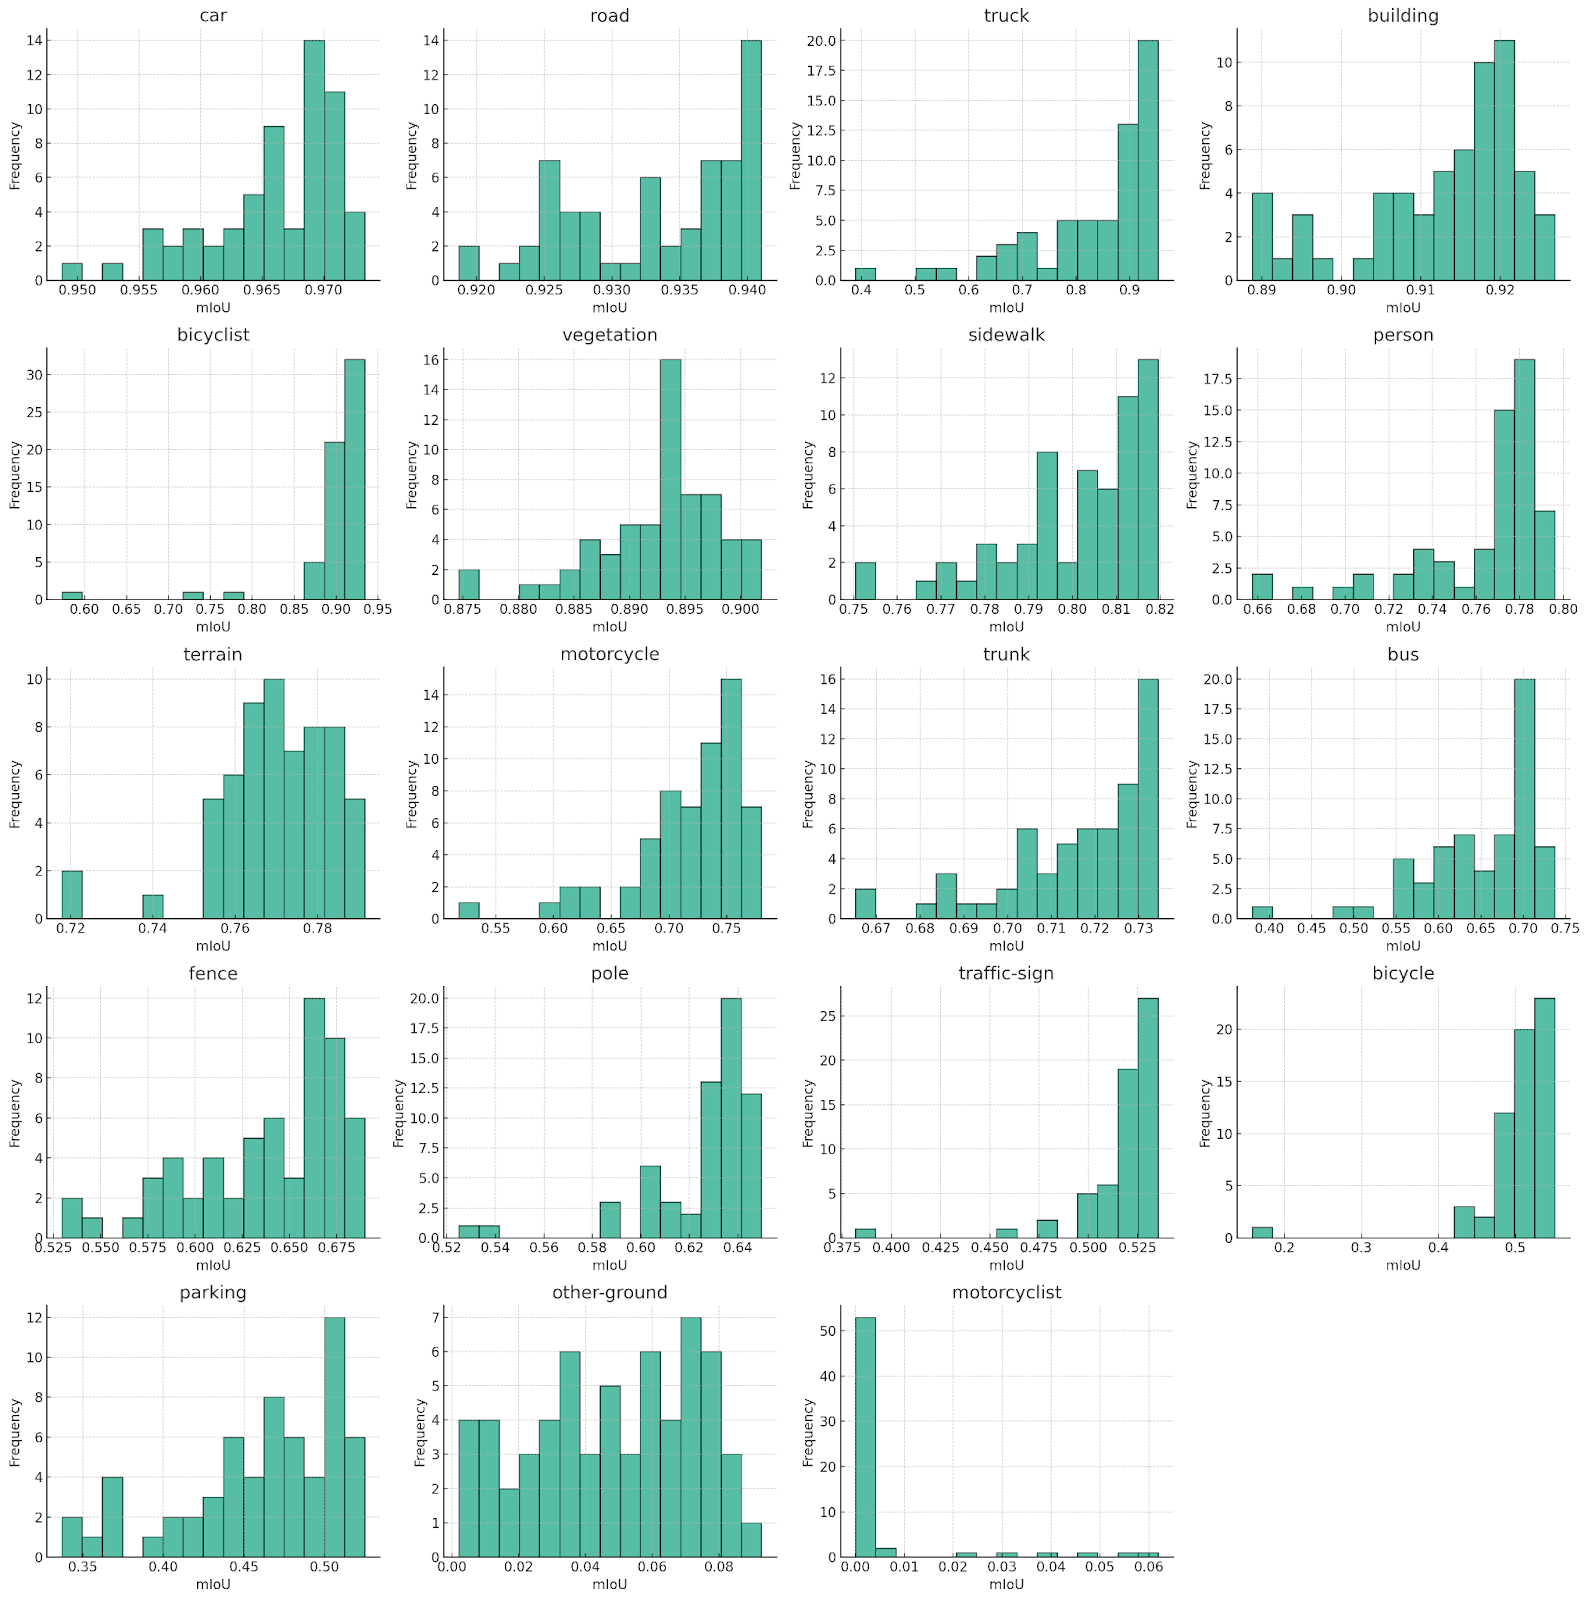
\includegraphics[width=0.5\textwidth]{photos/histogram of each class miou accross checkpoints.png}
    \caption{Class histogram miou accross collected training checkpoints for semantic Kitti dataset  }
    \label{fig:photo_example}
\end{figure}

\begin{table}[!h]
\centering
\begin{tabular}{l l}
\hline
\textbf{Class} & \textbf{Distribution} \\
\hline
Truck & Log-Normal \\
Bicyclist & Log-Normal \\
Person & Log-Normal \\
Bus & Log-Normal \\
Fence & Log-Normal \\
Pole & Log-Normal \\
Traffic-Sign & Log-Normal \\
Bicycle & Log-Normal \\
Motorcyclist & Log-Normal \\
\hline
\textbf{Remaining classes} & Normal distribution \\
\hline
\end{tabular}
\caption{Distribution of Classes' Scores}
\label{tab:scores_distribution}
\end{table}



\begin{figure}[!h]
    \centering
    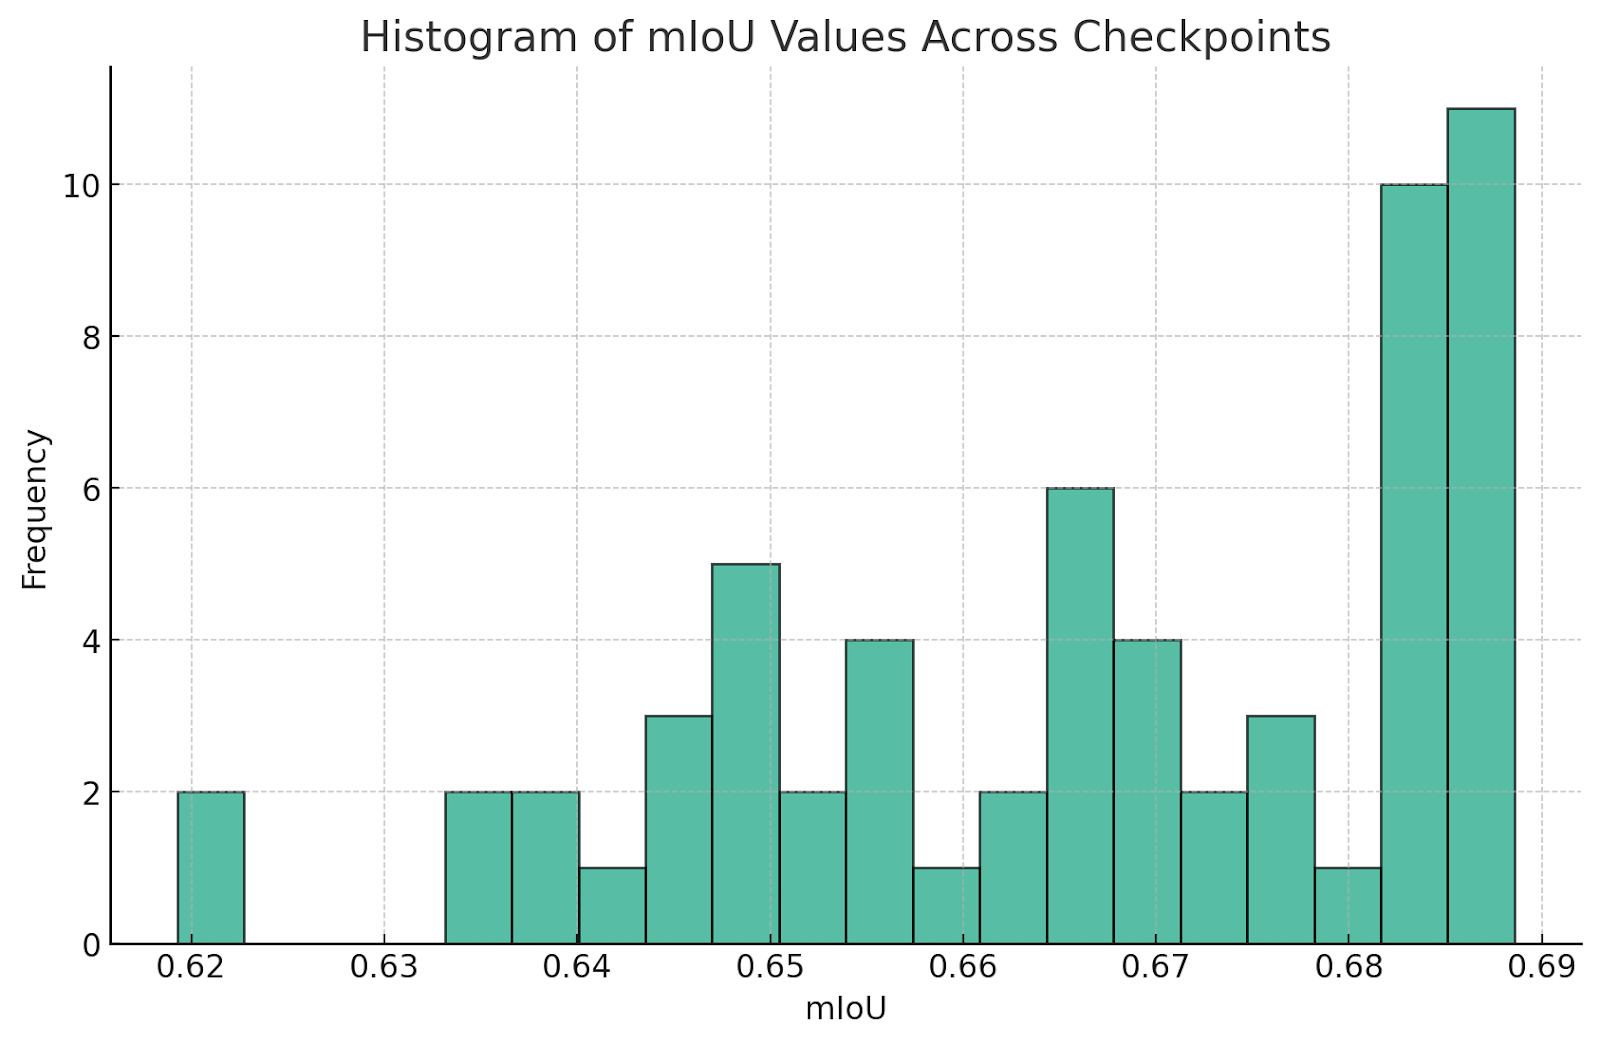
\includegraphics[width=0.5\textwidth]{photos/histogram of average miou of collected semantic kitti checkpoints.png}
    \caption{histogram of average histogram miou across collected training checkpoints for semantic Kitti dataset  }
    \label{fig:photo_example}
\end{figure}

Normal distribution of average mu over collected checkpoints 





\begin{figure}[!h]
    \centering
    \includegraphics[width=0.5\textwidth]{photos/miou_improvement_using_tta_num_of_votes_12.png}
    \caption{Class-wise performance improvement when using tta (num of votes = 12 ) vs not using tta}
    \label{fig:photo_example}
\end{figure}


\begin{table}[!h]
\centering
\begin{tabular}{l c}
\hline
Class & Average mIoU Improvement (\%) \\
\hline
Car & 1.04 \\
Road & 2.10 \\
Truck & 12.62 \\
Building & 1.72 \\
Bicyclist & 4.48 \\
Vegetation & 1.40 \\
Sidewalk & 3.51 \\
Person & 5.99 \\
Terrain & 2.02 \\
Motorcycle & 4.88 \\
Trunk & 2.82 \\
Bus & 7.78 \\
Fence & 5.72 \\
Pole & 5.66 \\
Traffic-Sign & 3.56 \\
Bicycle & 5.26 \\
Parking & 5.35 \\
Other-Ground & 1.30 \\
Motorcyclist & 0.05 \\
\hline
\textbf{All classes average improvement} & \textbf{4.07} \\\hline
\end{tabular}
\caption{Class-wise Average mIoU Improvements with Test-Time Augmentation (TTA)}
\label{tab:tta_miou_improvements}
\end{table}


\begin{table}[!h]
\centering
\begin{tabular}{l l}
\hline
\textbf{Class} & \textbf{Top 3 Checkpoints} \\
\hline
Car & [(39, 0.973), (11, 0.973), (21, 0.972)] \\
Road & [(18, 0.941), (16, 0.941), (13, 0.941)] \\
Truck & [(7, 0.953), (12, 0.950), (27, 0.947)] \\
Building & [(34, 0.927), (15, 0.926), (27, 0.924)] \\
Bicyclist & [(21, 0.934), (8, 0.929), (40, 0.927)] \\
Vegetation & [(20, 0.902), (36, 0.901), (26, 0.901)] \\
Sidewalk & [(18, 0.820), (16, 0.819), (8, 0.818)] \\
Person & [(38, 0.796), (24, 0.791), (41, 0.791)] \\
Terrain & [(20, 0.791), (34, 0.789), (24, 0.789)] \\
Motorcycle & [(4, 0.780), (3, 0.778), (32, 0.777)] \\
Trunk & [(7, 0.734), (8, 0.734), (23, 0.733)] \\
Bus & [(21, 0.738), (11, 0.732), (9, 0.720)] \\
Fence & [(37, 0.690), (27, 0.685), (9, 0.681)] \\
Pole & [(36, 0.650), (24, 0.649), (53, 0.644)] \\
Traffic-Sign & [(25, 0.535), (37, 0.535), (5, 0.534)] \\
Bicycle & [(42, 0.551), (9, 0.540), (37, 0.540)] \\
Parking & [(11, 0.525), (23, 0.519), (16, 0.519)] \\
Other-Ground & [(14, 0.093), (17, 0.085), (22, 0.084)] \\
Motorcyclist & [(31, 0.062), (30, 0.054), (55, 0.049)] \\
\hline
\end{tabular}
\caption{Top 3 Checkpoints for Each Class}
\label{tab:top_checkpoints}
\end{table}

\begin{table}[!h]
\centering
\begin{tabular}{l l}
\hline
\textbf{Checkpoint} & \textbf{Frequency} \\
\hline
11, 21, 16, 27, 8, 24, 9, 37 & 3 times each \\
18, 7, 34, 20, 36, 23 & 2 times each \\
\hline
\end{tabular}
\caption{Frequently Appearing Checkpoints in Top 3 for Each Class}
\label{tab:frequent_checkpoints}
\end{table}

The checkpoints that appear most frequently in the top 3 for each class are:
Checkpoints 11, 21, 16, 27, 8, 24, 9, and 37 each appear 3 times.
Checkpoints 18, 7, 34, 20, 36, and 23 each appear 2 times.

\subsection{Ablation study}

\begin{table}[!h]
\centering
\small
\begin{tabular}{|l|l|l|}
\hline
\textbf{Ingredients} & \textbf{Count} & \textbf{MIoU (\%)} \\
\hline
$[0]$ & 1 & 65.2798 \\
$[0,3]$ & 2 & 65.3449 \\
$[0,3,7]$ & 3 & 65.5071 \\
$[0,3,7,12]$ & 4 & 65.6145 \\
$[0,3,7,12,18]$ & 5 & 65.6381 \\
$[0,3,7,12,18,19]$ & 6 & 65.9205 \\
$[0,3,7,12,18,19,20]$ & 7 & 66.0292 \\
$[0,3,7,12,18,19,20,22]$ & 8 & 66.0755 \\
$[0,3,7,12,18,19,20,22,23]$ & 9 & 66.1055 \\
$[0,3,7,12(2),18,19,20,22,23]$ & 10 & 66.1087 \\
$[0,3,7,12(2),18(2),19,20,22,23]$ & 11 & 66.1551 \\
$[0,3,7,12(2),18(2),19,20,22,23(2)]$ & 12 & 66.1691 \\
$[0,3,7,12(2),18(3),19,20,22,23(2)]$ & 13 & 66.1711 \\
$[0,3,7,12(2),18(3),19,20,22(2),23(2)]$ & 14 & 66.2202 \\
\hline
\end{tabular}
\caption{semantic Kitti MIoU values for different ingredient combinations}
\end{table}

\begin{figure}[!h]
    \centering
    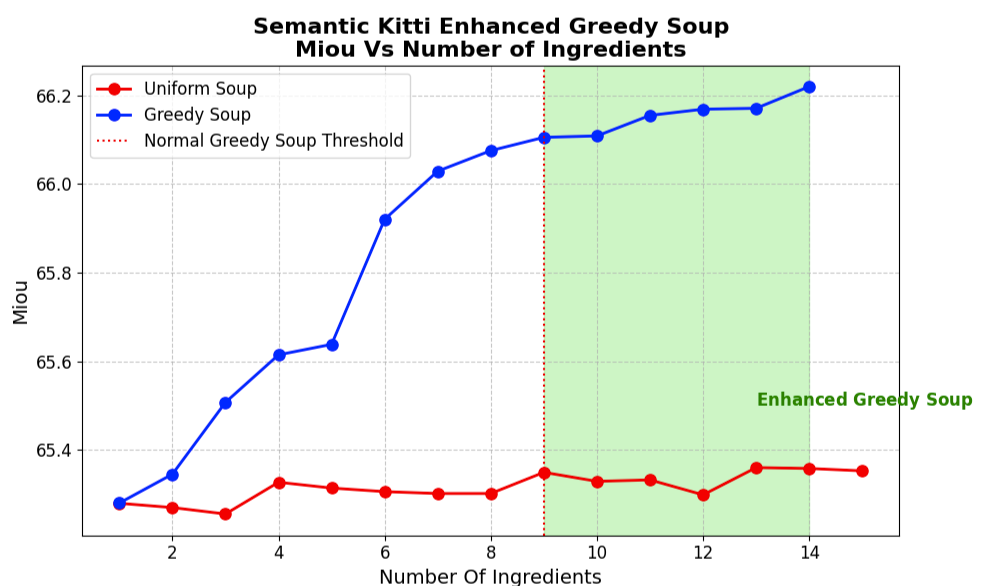
\includegraphics[width=0.5\textwidth]{photos/semantickitti_soup.png}
    \caption{Enhaced Greedy Soup improves 1\% on best checkpoint }
    \label{fig:photo_example}
\end{figure}
\begin{table}[!h]
\centering
\small
\begin{tabular}{|l|l|l|}
\hline
\textbf{Ingredients} & \textbf{Count} & \textbf{MIoU (\%)} \\
\hline
$[0]$ & 1 & 75.7099\\
$[0,1]$ & 2 & 75.8291\\
$[0,1,2]$ & 3 & 75.8732 \\
$[0,1,2,3]$ & 4 & 75.9178 \\
$[0,1,2,3,4]$ & 5 & 76.0154 \\
$[0,1,2,3,4,15]$ & 6 & 76.0245 \\
$[0,1,2,3,4,15,21]$ & 7 & 76.0398 \\
$[0,1,2,3,4,15,21,29]$ & 8 & 76.0656 \\
$[0,1,2,3,4,15,21,29,66]$ & 9 & 76.0809 \\
$[0,1,2,3,4,15,21,29,66,73]$ & 10 & 76.0812 \\
$[0(2),1,2,3,4,15,21,29,66,73]$ & 11 & 76.0912 \\
$[0(2),1(2),2,3,4,15,21,29,66,73]$ & 12 & 76.1110 \\
$[0(2),1(2),2,3,4(2),15,21,29,66,73]$ & 13 & 76.1297 \\
$[0(2),1(2),2,3,4(2),15,21(2),29,66,73]$ & 14 & 76.1323 \\
$[0(2),1(2),2,3,4(2),15,21(2),29(2),66,73]$ & 15 & 76.1368 \\
\hline
\end{tabular}
\caption{Nuscenes MIoU values for different ingredient combinations}
\end{table}


\begin{figure}[!h]
    \centering
    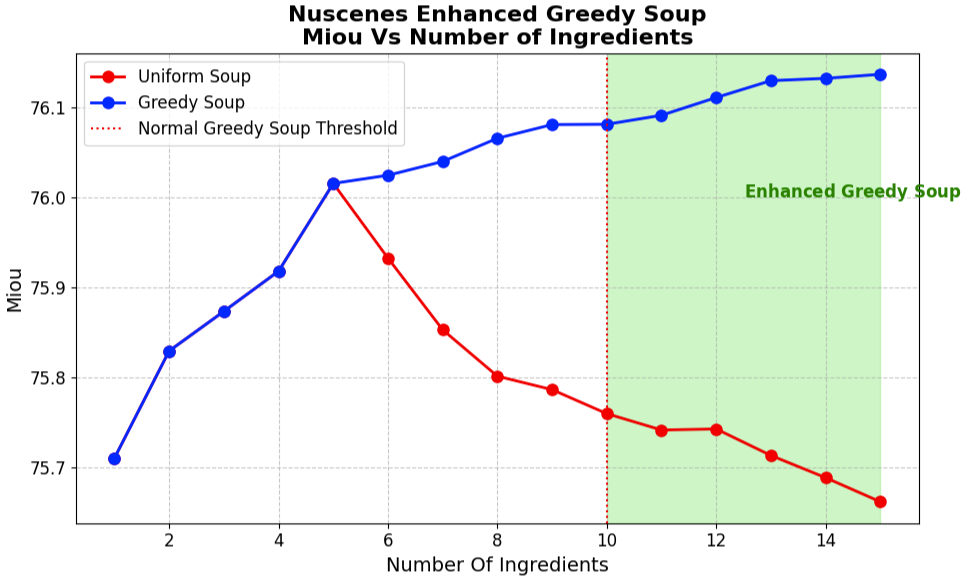
\includegraphics[width=0.5\textwidth]{photos/nuscenes_soup.png}
    \caption{Enhaced Greedy Soup improves 0.5\% on best checkpoint }
    \label{fig:photo_example}
\end{figure}




\section{Conclusion}
We introduce a new method named "Iterative Scan Greedy Model Soup" that we have applied to LiDAR semantic segmentation. By harnessing this innovative approach, we enhance an advanced open-source 2DPASS \cite{yan20222dpass} semantic segmentation code and showcase its effectiveness on the semantic Kitti and nuscenes datasets. Significantly, our technique achieves remarkable enhancements in Mean Intersection Over Union (MIoU) metrics, all while maintaining the prediction time unchanged.



\bibliographystyle{plain} % Choose a bibliography style
\bibliography{egbib} % Specify the .bib file name without the extension
\end{document}
